\documentclass[12pt,letterpaper]{article}
\usepackage[margin=1in]{geometry}
\usepackage{fancyhdr}
\usepackage[utf8]{inputenc}
\usepackage{palatino}
\usepackage{microtype}
\usepackage{hyperref}
\usepackage{graphicx}
\usepackage[hang,bf,small]{caption}
\usepackage{amsmath,amssymb,amsthm}

\setlength{\parindent}{0cm}
\setlength{\parskip}{1em}

\hypersetup{colorlinks,
	linkcolor = black,
	citecolor = black,
	urlcolor  = black}
\urlstyle{same}

\begin{document}

\begin{titlepage}
	\vspace*{4cm}
	\begin{flushright}
	{\huge
		Cattlestar Balactica \\ [1cm]
	}
	{\large
		ENGR 421 -- Week 5 Individual Lab Report \\ [3cm]
	}
	\end{flushright}

	\begin{flushright}
	2 May 2013 \\
	Soo-Hyun Yoo
	\end{flushright}

\end{titlepage}

\newpage

\section*{Done}

\subsection*{PI Control}

The BB shooter regulates the velocity of the flywheel using a PI controller.
Interestingly, the I term seems to do most of the heavy work of maintaining
wheel speed than the P term.

\subsection*{GUI}

I wrote a simple GUI with Qt and C++ that integrates with ROS, shown below. The
number fields allow me to configure thresholds for the fledgling vision
software.

\begin{figure}[!h]
	\centering
	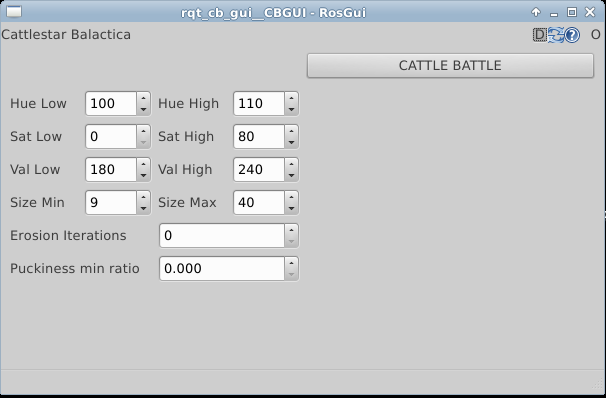
\includegraphics[width=0.6\textwidth]{gui.png}
	\caption{Qt GUI.}
	\label{fig:gui}
\end{figure}

\subsection*{Puck detection}

I can now detect a triangular puck and its location regardless of orientation.
I have neither implemented rectification of the board nor specified any regions
of interest, so noise from outside the board space is proving to be a big
issue. This will be solved this weekend by extracting corner points from the
board (via more color filtering) and using them with OpenCV's
perspectiveTransform function.

\begin{figure}[!h]
	\centering
	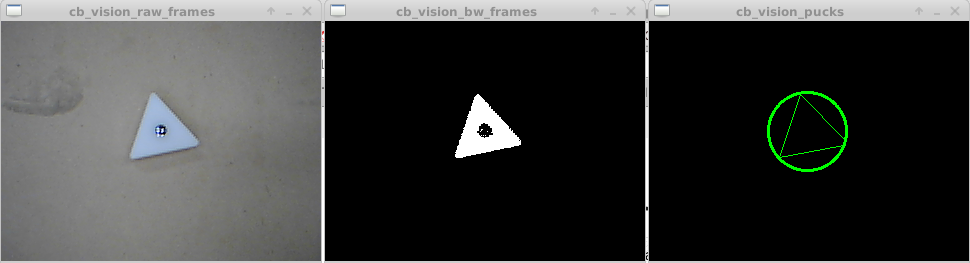
\includegraphics[width=0.9\textwidth]{puck1.png}
	\caption{Puck recognized from above.}
	\label{fig:puck1}
\end{figure}

\begin{figure}[!h]
	\centering
	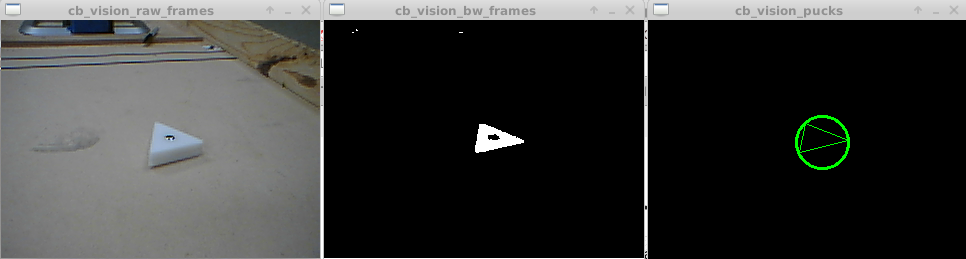
\includegraphics[width=0.9\textwidth]{puck2.png}
	\caption{Puck recognized from an angle.}
	\label{fig:puck2}
\end{figure}

\begin{figure}[!h]
	\centering
	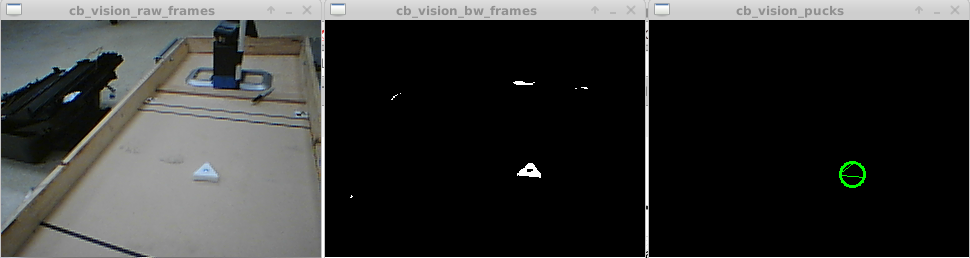
\includegraphics[width=0.9\textwidth]{puck3.png}
	\caption{Puck recognized from farther away with noise.}
	\label{fig:puck3}
\end{figure}


\section*{Todo}

This weekend and much of next week will be spent nailing down puck detection
and targeting. I hope to achieve a jitter of less than 2 cm when the puck is at
the far end of the board. This may require operating the webcam at its 640x480
mode.

I still need to program the linear rail system, but that is of much lower
priority compared to the vision system. (Additionally, the software
architecture for controlling the rails is already in place, so it's actually
pretty much done.)

\end{document}

